\documentclass[border=0.125cm]{standalone}
\usepackage{tikz}
\usetikzlibrary{positioning}

\begin{document}


\tikzset{%
  every neuron/.style={
    circle,
    draw,
    minimum size=1cm
  },
  neuron missing/.style={
    draw=none, 
    scale=4,
    text height=0.333cm,
    execute at begin node=\color{black}$\vdots$
  },
}

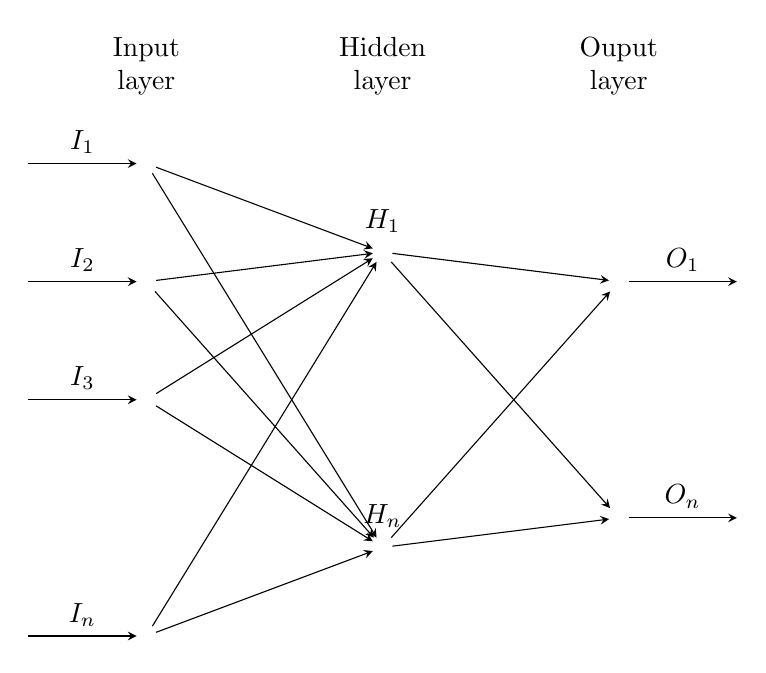
\begin{tikzpicture}[x=1.5cm, y=1.5cm, >=stealth]

	% input layer
	\foreach \m/\l [count=\y] in {1,2,3,missing,4}
	  \node [every neuron/.try, neuron \m/.try] (input-\m) at (0,2.5-\y) {};
	
	% hidden layer
	\foreach \m [count=\y] in {1,missing,2}
	  \node [every neuron/.try, neuron \m/.try ] (hidden-\m) at (2,2-\y*1.25) {};
	
	% output layer
	\foreach \m [count=\y] in {1,missing,2}
	  \node [every neuron/.try, neuron \m/.try ] (output-\m) at (4,1.5-\y) {};
	
	% labels for input layer
	\foreach \l [count=\i] in {1,2,3,n}
	  \draw [<-] (input-\i) -- ++(-1,0)
	    node [above, midway] {$I_\l$};
	
	% labels for hidden layer
	\foreach \l [count=\i] in {1,n}
	  \node [above] at (hidden-\i.north) {$H_\l$};
	
	% labels for output layer
	\foreach \l [count=\i] in {1,n}
	  \draw [->] (output-\i) -- ++(1,0)
	    node [above, midway] {$O_\l$};
	
	% connections for input layer
	\foreach \i in {1,...,4}
	  \foreach \j in {1,...,2}
	    \draw [->] (input-\i) -- (hidden-\j);
	
	% connections for hidden to output layer
	\foreach \i in {1,...,2}
	  \foreach \j in {1,...,2}
	    \draw [->] (hidden-\i) -- (output-\j);
	
	% labels for each layer at the top
	\foreach \l [count=\x from 0] in {Input, Hidden, Ouput}
	  \node [align=center, above] at (\x*2,2) {\l \\ layer};

\end{tikzpicture}

\end{document}
